\section{Model}
\label{sec:model}

In this section we first formally define snapshot graphs, and then
show how graph evolution is represented by assigning temporal meaning
to sequences of snapshot graphs.

\begin{definition}[Snapshot graph]
\label{def:sg} 
A {\em snapshot graph} (or a {\em snapshot}) is a pair $G = (V,E)$,
where $V$ is a finite set of nodes with schema $(\underline{vid},
a_1, \ldots, a_n)$, and $E$ is a finite set of edges connecting
pairs of nodes from $V$, with schema $(\underline{vid_1},
\underline{vid_2}, a_1, \ldots, a_m)$.
\end{definition}

\begin{figure}
\label{fig:sg}
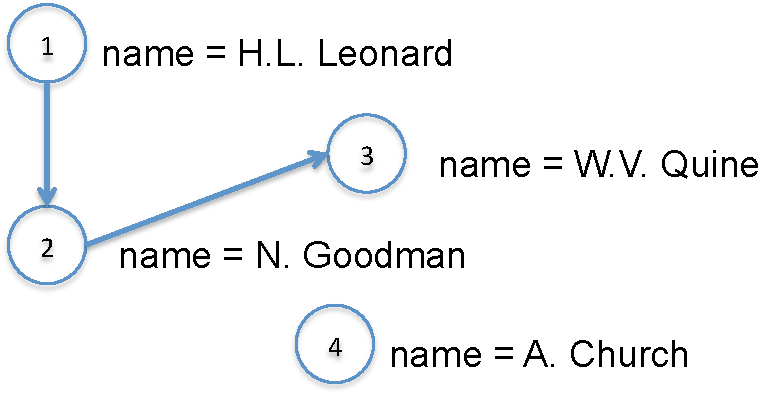
\includegraphics[width=3.2in]{figs/snapshot.pdf}
\caption{Snapshot of VLDB co-authorship graph for 1940, with a single string node attribute $name$ and no edge attributes.}
\end{figure}

Attributes of vertices and of edges are not restricted to be of atomic
types, but may, e.g., be maps or tuples. However it is required that
all vertices (resp. edges) of $G$ have the same schema, i.e., $V$ and
$E$ are homogeneous sets.

\begin{definition} [Structural union-compatibility]
\label{def:scompat}
Snapshot graphs $G' = (V', E')$ and $G'' = (V'', E'')$ are
union-compatible if $V'$ and $V''$ are union-compatible, and $E'$ and
$E''$ are union-compatible.
\end{definition}

This is a standard union compatibility definition, which requires the
vertex schma $V$ to be the same for both graphs $G'$ and $G''$ (same
for edge schema $E$).  For example, the snapshot in
Figure~\ref{fig:sg} is only compatible with other snapshots where
vertices have one string attribute $name$ and no edge attributes.

$G$ may represent a directed or an undirected graph.  For undirected
graphs we choose a canonical representation of an edge, with $vid_1
\leq vid_2$ (self-loops are allowed).

We next describe how time is represented in our model.  Following the
SQL:2011 standard~\cite{DBLP:journals/sigmod/KulkarniM12}, we adopt
the {\em closed-open} period model, i.e., a period represents all
times starting from and including the start time, continuing to but
excluding the end time.

\begin{definition}[Time period]
\label{def:period} 
A {\em time period} \\$p = [start, end)$ is an interval on the timeline,
  subject to the constraint $start < end$.  We refer to the length of
  time covered by $p$ as its {\em resolution}.
\end{definition}

We focus on {\em valid time}, represented by {\em application-time
  period} in SQL:2011 --- the time period during which data is
regarded as correctly reflecting reality.  This is in contrast to {\em
  transaction time} (or {\em system-time period}), which refers to the
time period during which a row is committed to the database.  Our goal
in this work is to support complex analytics over evolving graphs,
under the assumption that all historical data is available in the
database and is read-only.

We represent graph evolution by associating a sequence of snapshots,
which are not themselves time-aware, with a a sequence of time
periods.  This is stated formally next.

\begin{definition} [Temporal sequence]
\label{def:tseq} 
A {\em temporal sequence} $P = (p_1, \ldots, p_n)$ is a
sequence of consecutive non-overlapping time periods of the same
resolution, with no gaps.  That is,

\begin{enumerate}
\item $\forall i < n, p_i.end = p_{i+1}.start$, and 
\item $\forall i, j, p_i.end - p_i.start = p_j.end - p_j.start$.
\end{enumerate}
\end{definition}

$P$ may be equivalently described by 3 values: the start of the
earliest period $P.start = p_1.start$, the end of the latest period
$P.end = p_n.end$, and the resolution of any period $P.res = p_1.end -
p_1.start$. For convenience, we refer to the number of periods in the
sequence as $P.size$.  

For example, $[1940,1945), [1945,1950), … [2010,2015)$ represents a
      temporal sequence in the interval [1940,2015) with size 15 and
        resolution 5.

\julia{Define the null sequence: what are the start / end /
  resolution, considering that $start < end$, not $start \leq end$.}

\vera{According to the wiki, $[a,a)$ is considered an empty set. So if
    we just follow the standard interval math semantics, we can say: A
    null temporal sequence is a sequence represented by the
    $[p.start,p.end)$ time interval regardless of the resolution. By
      definition it is of size 0.}

We adopt a SQL 2011 temporal predicate definitions for {\em contains},
{\em overlaps}, {\em equals}, {\em preceeds}, and {\em succeeds} for
time periods.  We further define these predicates for a temporal
sequence by reducing it to the $p_1.start$ and $P_n.end$ time
interval.  I.e., a temporal sequence $P'$ preceeds temporal sequence
$P''$ if $P'.p_n.end \leq P''.p_1.start$.

\begin{definition} [Temporal Sequence Interval Intersection]
\label{def:tseqii}
The intersection of a temporal sequence $P$ and interval
$[p.start,p.end)$ is a subset $P'$ with $P'.start = max(P_1.start,
  P_i.start), P'.end = min(P_n.end, P_j.end)$, where $P_i$ immediately
  succeeds $p.start$ and $P_j$ immediately preceeds $p.end$.
\end{definition}

\vera{I am not sure whether immediately succeeds/preceeds includes a
  full match, i.e. [1,2) and start=1 should include [1,2) in the
      result.}

For example, the intersection of temporal sequence $[3,5),[5,7),[7,9)$
      and time interval $[1,8)$ is $[3,5),[5,7)$. $[7,9)$ is not
              included because 8 is in the middle of that interval and
              cannot be included fully.

\begin{definition} [Temporal Union-Compatibility]
\label{def:tcompat} 
Temporal sequences $P'$ and $P''$ are union-compatible if they have
the same resolution, and if we can construct a valid temporal sequence
$P$ with $P.start = min(P'.start, P''.start)$, $P.end = max(P'.start,
P''.start)$, and with $P.res = P'.res$.
\end{definition}

For example, consider these 4 sequences:
\begin{enumerate}
\item $[1,3),[3,5),[5,7),[7,9)$
\item $[9,10),[10,11)$
\item $[8,10),[10,12),[12,14)$
\item $[15,17),[17,19)$
\end{enumerate}

Sequence 2 is not union-compatible with any other because it has a
different resolution.  Sequences 1 and 3 are not union-compatible
because, while the resolution is the same, [1,14) is not a valid
  temporal sequence of resolution 3.  Finally, sequences 1 and 4 are
  union-compatible.  Notice that there is no requirement for the two
  sequences to be consecutive to be union-compatible. We describe a
  result of two non-consecutive temporal sequences further in this
  section.

\begin{definition} [Temporal Sequence Overlap]
\label{def:tseqoverlap}
Temporal overlap between two union-compatible temporal sequences $P'$
and $P''$ is an intersection $P' \cap P''$ of time periods comprising
$P'$ and $P''$.
\end{definition}

Recall that a snapshot represents a single state of an evolving graph,
and is not itself time-aware.  Temporal evolution of a graph is
represented by a sequence of snapshots, called {\em temporal graphs}
in our formalism. 

\begin{definition} [Temporal Graph]
\label{def:tgraph} 
A {\em temporal graph} $T = (G_1, \ldots, G_n; P)$ associates a
sequence of $n$ structurally union-compatible snapshots with a
temporal sequence $P$, such that $P.size = n$.
\end{definition}

Snapshot graphs in the sequence define the {\em structural schema} of
$T$, while the {\em temporal schema} of $T$ is specified by $P$.
Identity of a vertex persists across snapshots in a temporal graph,
and across temporal graphs.

For example, in Figure~\ref{fig:tgraph} vertex with id 3 represents
the same author W. V. Quine, who published a paper in both of those
time periods.

\begin{figure}
\label{fig:tgraph}
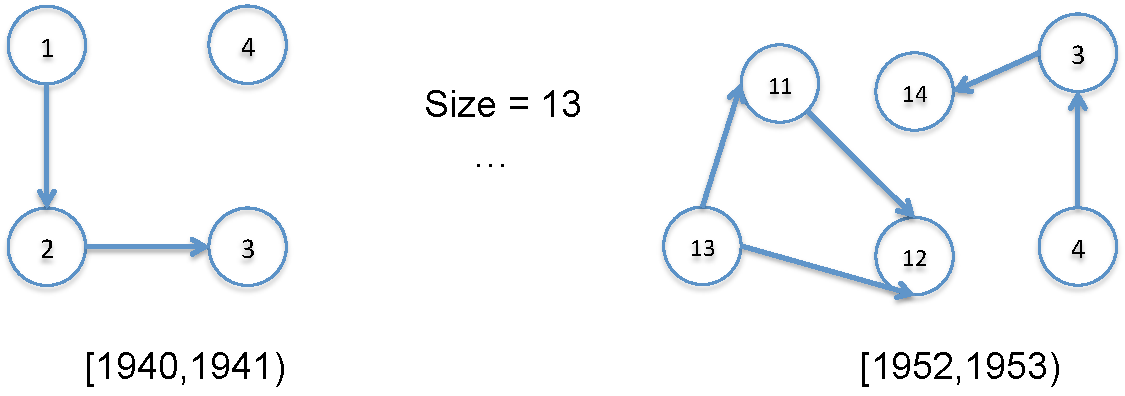
\includegraphics[width=3.2in]{figs/temporalgraph.pdf}
\caption{A temporal graph of VLDB co-authorship over the period from 1940 to 1953.}
\end{figure}

A  temporal graph of Definition~\ref{def:tgraph} is the basic
element in our model.  In what follows, we assume that a relation in
our database corresponds to a single temporal graph, not to a
collection of temporal graphs.  In the next section we will define a
temporal graph query language \ql, in which operators take as input a
single temporal graph or a pair of temporal graphs, and produce a
temporal graph as output.

To support binary operations, we now define union compatibility of
temporal graphs.

\begin{definition} [Graph Union-Compatibility]
\label{def:tuc} Temporal graphs $T'$ and $T''$ are union-compatible if they are both
structurally union-compatible (per Definition~\ref{def:scompat}) and
temporally union-compatible (per Definition~\ref{def:tcompat}).
\end{definition}




